\documentclass{article}

\usepackage{enumitem}
\usepackage{amsmath}
\usepackage{amsfonts}
\usepackage{amssymb}
\usepackage{amsthm}
\usepackage{algorithm}
\usepackage{algorithmic}
\usepackage[margin=0.5in]{geometry}
\usepackage[hidelinks, bookmarks=false]{hyperref}

\usepackage[dvipsnames]{xcolor}

\let\oldemptyset\emptyset
\let\emptyset\varnothing
\newcommand{\R}{\mathbb{R}}
\newcommand{\Rd}{\R^d}

\usepackage{environ}
\NewEnviron{centerframebox}{\begin{center}\fbox{\parbox{0.92\textwidth}{\BODY}}\end{center}}

\title{Discrete and Computational Geometry \\ Assignment 9}
\author{
  \AA{AAAAAAAAAA AAAAAAA}{6} \\
  \href{mailto:\AA{AAAAAAAAAAAAAAAAAAAA}{7}}{\AA{AAAAAAAAAAAAAAAAAAAA}{7}}
  \and
  Ayush Mishra \\
  \href{mailto:s28amish@uni-bonn.de}{s28amish@uni-bonn.de}
}

\usepackage{graphicx}
\graphicspath{{./} {img/}}

\usepackage{titlesec}
\titleformat{\section}
  {\normalfont\Large\bfseries}{Problem \thesection : }
  {0em}{\mdseries}

\begin{document}
  \maketitle
  \begin{center}
    { \bfseries Deadline: 20 Dec 2024, 23:55 }
  \end{center}

  \section{}
  \begin{centerframebox}
    Consider the example of 4 line segments in Figure 1 on the next page. Let $s_1, \ldots, s_4$ be the permutation of line segments used in Algorithm 16.1.

    \begin{enumerate}[label=(\alph*)]
      \item Draw the current state of the trapezodial decomposition computed by the algorithm after each iteration of the for-loop.
      \item Draw the search graph $G$ computed by the algorithm after each iteration of the for-loop.
    \end{enumerate}
  \end{centerframebox}
  \subsection{(a)}
  \begin{center}
    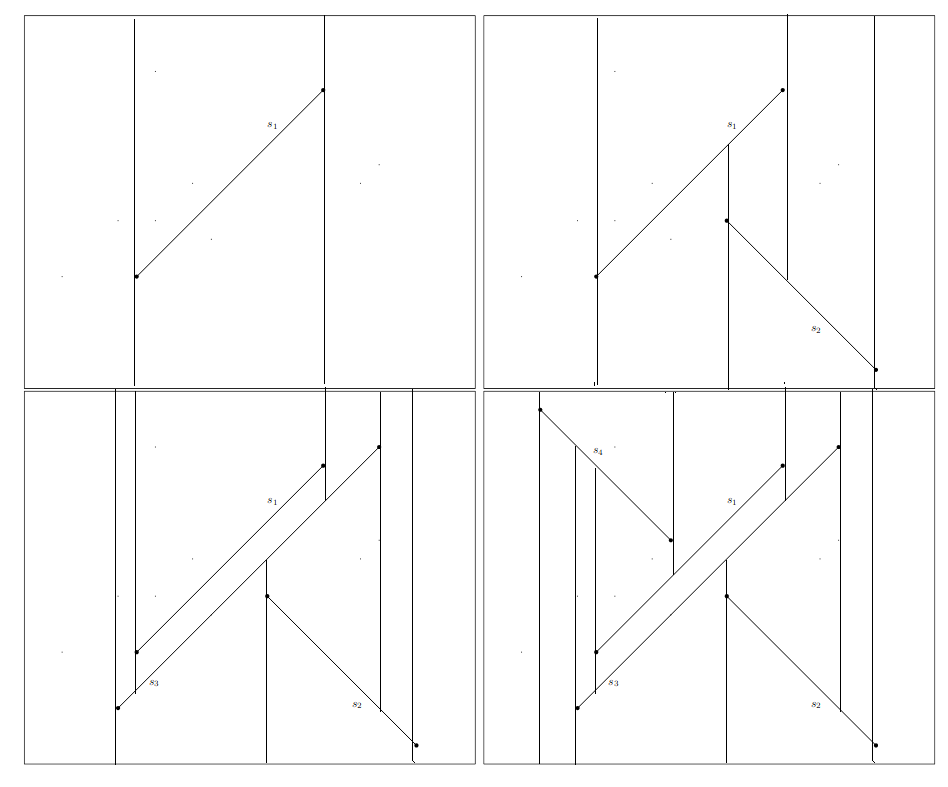
\includegraphics[width=.7\textwidth]{trapezoidal-1}

    Figure 1: The trapezodial decomposition after each iteration
  \end{center}

  \subsection{(b)}
  \begin{center}
    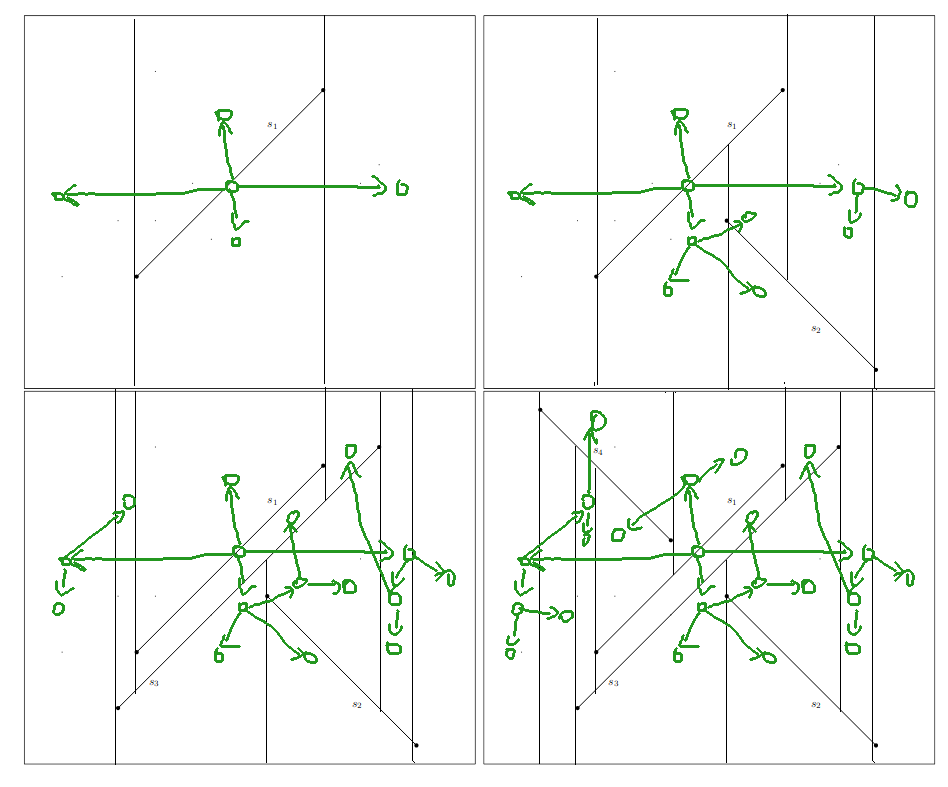
\includegraphics[width=.7\textwidth]{trapezoidal-2}

    Figure 2: The search graph after each iteration
  \end{center}

  \section{}
  \begin{centerframebox}
    Consider Algorithm 16.1 from Lecture 16. The algorithm needs to find the faces $f_2, \ldots, f_k$ that properly intersect $s_i$ in line 7. Show that the expected number of faces $k$ that properly intersect $s_i$ is in $O(1)$.

    \smallskip
    \textbf{Hint}: Use backwards analysis.
  \end{centerframebox}
  \newpage
  \section{}
  \begin{centerframebox}
    Let $P \subset \mathbb{R}^2$ be a \textit{star-shaped} polygon. That means there exists a kernel point $p \in P$ such that for every point $r \in P$ the line segment $\overline{pr}$ is contained in $P$. For an example of a star-shaped polygon see Figure 2 on the next page. Let $p_1, \ldots, p_n \in \mathbb{R}^2$ be the vertices of the boundary of $P$ in counterclockwise order. Design an algorithm that takes the ordered sequence $p_1, \ldots, p_n$ and the kernel point $p$ as input and computes a triangulation of $P$ in $O(n)$ time. You may assume that each star shaped polygon with kernel point $p$ and more than three vertices $p_1, \ldots, p_n$ contains a vertex $p_i$ such that the quadrilateral $p, p_{i-1}, p_i, p_{i+1}$ is convex.
  \end{centerframebox}

    We can think of a simple linear time algorithm for triangulating a star-shaped polygon $P$ by exploiting its geometric properties. Given a kernel point $p$ and vertices $p_1,\ldots,p_n$ in counterclockwise order, we can construct a valid triangulation through careful vertex removal while maintaining the star-shaped property.

    The algorithm works as follows:
    \bigskip
    \begin{algorithmic}
    \REQUIRE Kernel point $p$, vertices $p_1,\ldots,p_n$ in counterclockwise order
    \ENSURE Triangulation $T$ of the star-shaped polygon $P$
    \STATE $T \leftarrow \emptyset$
    \WHILE{$n > 3$}
       \STATE Find $p_i$ where quadrilateral $(p,p_{i-1},p_i,p_{i+1})$ is convex
       \STATE $T \leftarrow T \cup \{\triangle pp_{i-1}p_i, \triangle pp_ip_{i+1}\}$
       \STATE Remove $p_i$ from vertex sequence and update indices
       \STATE $n \leftarrow n-1$
    \ENDWHILE
    \STATE $T \leftarrow T \cup \{\triangle pp_1p_2\}$
    \RETURN $T$
    \end{algorithmic}

    To prove correctness, note three key properties that hold throughout the algorithm:

    \begin{enumerate}
    \item All triangles added by the algorithm lie inside $P$. This follows directly from the star-shaped property --- for any vertex $v$, the line segment $\overline{pv}$ lies entirely in $P$. Since we only add triangles formed by $p$ and consecutive vertices on the polygon boundary, these triangles must lie within $P$.

    \item We can always make progress because, by the problem assumption, there exists a vertex $p_i$ such that the quadrilateral $(p,p_{i-1},p_i,p_{i+1})$ is convex. This ensures we can always find a valid vertex to remove.

    \item After removing vertex $p_i$ and its incident triangles, the remaining polygon is still star-shaped with respect to $p$. This is because:
       \begin{itemize}
       \item The removed triangles exactly cover the region between segments $\overline{pp_{i-1}}$, $\overline{pp_i}$, and $\overline{pp_{i+1}}$
       \item The convexity of the quadrilateral ensures no self-intersections are created
       \item Any line segment $\overline{pr}$ from $p$ to a remaining vertex $r$ stays within the original polygon
       \end{itemize}
    \end{enumerate}

    For the running time analysis:
    \begin{itemize}
    \item Finding a valid vertex takes $O(1)$ time per check
    \item Each iteration removes one vertex and adds two triangles in constant time
    \item We perform exactly $n-3$ iterations
    \item All other operations (vertex removal, index updates) take constant time
    \end{itemize}

    Therefore, the total time complexity is $O(n)$. The space complexity is also linear as we only store the triangulation and current vertex sequence.

    The algorithm produces exactly $n-2$ triangles: each iteration adds two triangles and removes one vertex, except the final step which adds one triangle. With $n-3$ iterations plus the final triangle, we get $n-2$ triangles total, which is optimal for any polygon triangulation.

  % \begin{enumerate}
  %   \item Iterate over points $p_i \in p_1, \ldots, p_n$.
  %   \item If the line segment $p_ip_{i+2}$ is contained in $P$, add the triangle $p_ip_{i+1}p_{i+2}$ to the triangulation and remove it from $P$.
  %     This action preserves the star-shaped property of $P$, when removing the triangle from it, and continuing recursively.
  %     So the reminder of the algorithm will also work.
  %   \item If the line segment is not contained in $P$, we can skip to the next $i$. Eventually, such a line segment will be found, because of the assumption from the task, in which a convex quadrilateral must always exist.
  %   \item Stop once we reach a star-shaped polygon with 3 vertices. Also add it to the triangulation.
  % \end{enumerate}
  % This a $o(n)$ algorithm, because it will only consider each point on the boundary once. Even after removing triangles from $P$, we can keep using the same $i$ index.

\end{document}
